%# -*- coding:utf-8 -*-
\documentclass[10pt,aspectratio=169,mathserif]{beamer}		

\usepackage{zju}
\usepackage{amsmath,amsfonts,amssymb,bm}
\usepackage{color}
\usepackage{graphicx,hyperref,url}
\usepackage{metalogo}
% \usepackage{fontspec}
\usepackage{mathptmx}
\usepackage{times}
\usepackage{textcomp}
\usepackage{subcaption}
\usepackage{filecontents}
\usepackage[style=verbose,backend=biber]{biblatex}
\addbibresource{ref.bib}


\newcommand{\code}[1]{\texttt{{\detokenize{#1}}}}

\usefonttheme{serif}

\beamertemplateballitem

\title{DMAAUTH: A Lightweight Pointer Integrity-based Secure Architecture to Defeat DMA Attacks}

% \subtitle{Subtitle}			

\author{\textbf{Xingkai Wang}, Wenbo Shen, Yujie Bu, Jinmeng Zhou, Yajin Zhou}
  
\institute{Zhejiang University}

\date{\today{}}
  
\begin{document}

\begin{frame}
	\titlepage
\end{frame}

% \section{Outline}
\begin{frame}{Outline}
	\tableofcontents
\end{frame}

\section{Motivation}
\begin{frame}{Motivation}
	\begin{figure}
		\centering
		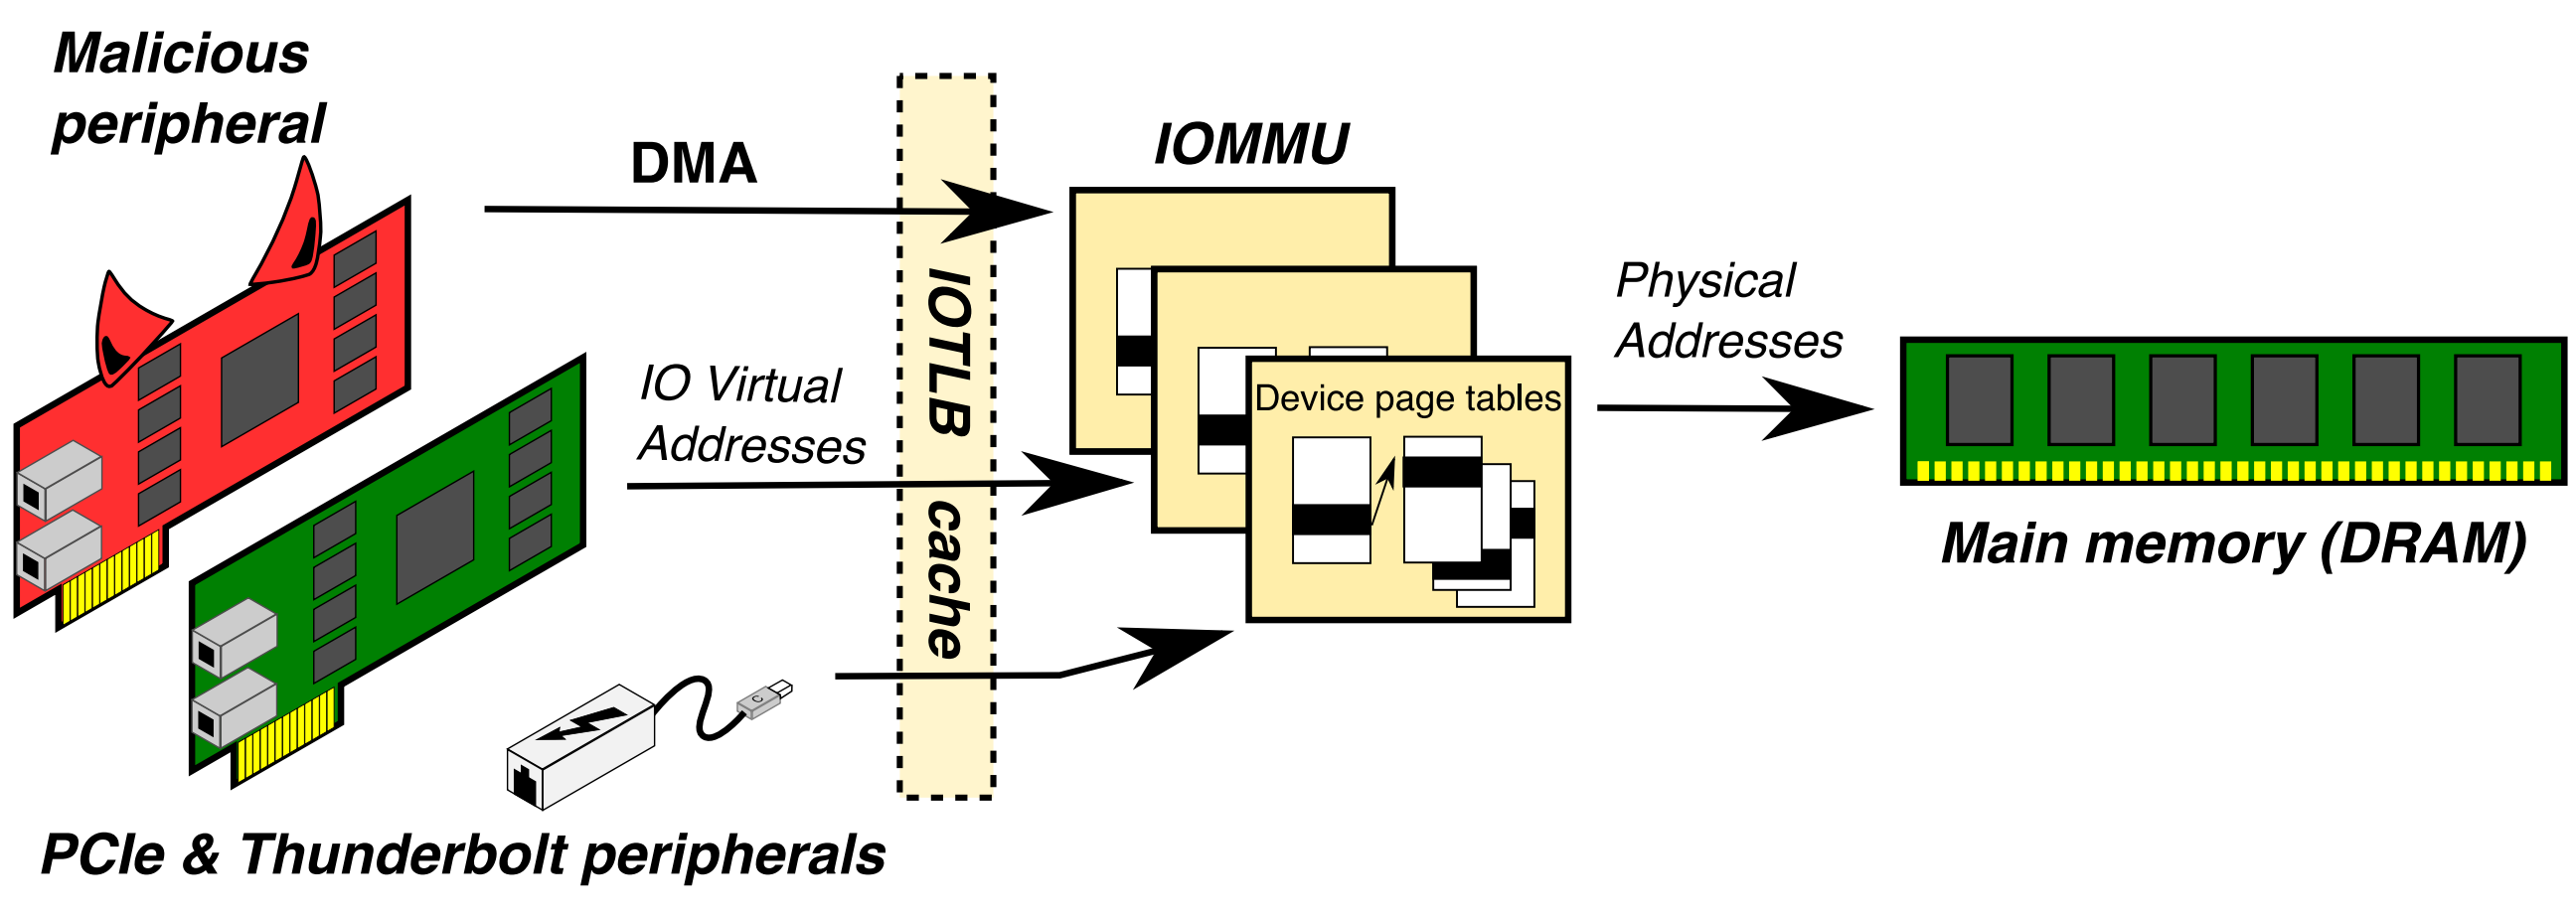
\includegraphics[width=\linewidth]{./images/motivation.png}
		\caption{Some peripherals (or the software running on them) should not be trusted.\footcite{thunderclap}}
	\end{figure}
\end{frame}

\section{Background}
\begin{frame}{Spatial Vulnerability}
	\begin{figure}
		\centering
		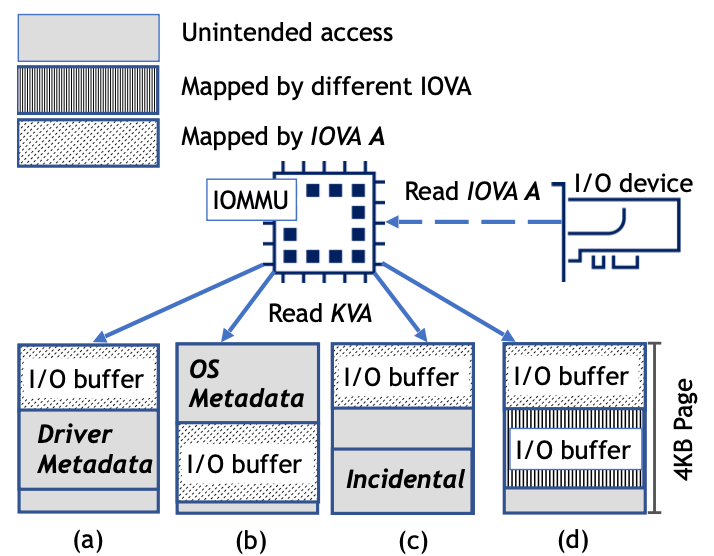
\includegraphics[width=0.45\linewidth]{./images/spatial.png}
		\caption{Page-granularity protection is not enough. Perihperals can still access the memory not for DMA. \footcite{char}}
	\end{figure}	
\end{frame}

\begin{frame}{Temporal Vulnerability}
	\begin{figure}
		\centering
		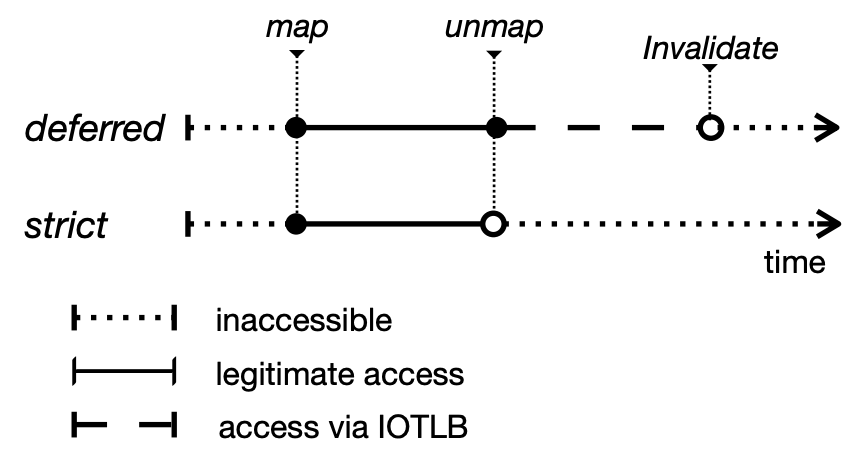
\includegraphics[width=0.6\linewidth]{./images/temporal.png}
		\caption{Peripherals can still access the memory after unmapping. Even if the kernel validates these memory regions after unmapping, the peripherals can still tampers with these regions.\footcite{char}}
	\end{figure}
\end{frame}

\begin{frame}{Existing Mechanisms}
	% \begin{figure}
	% 	\centering
	% 	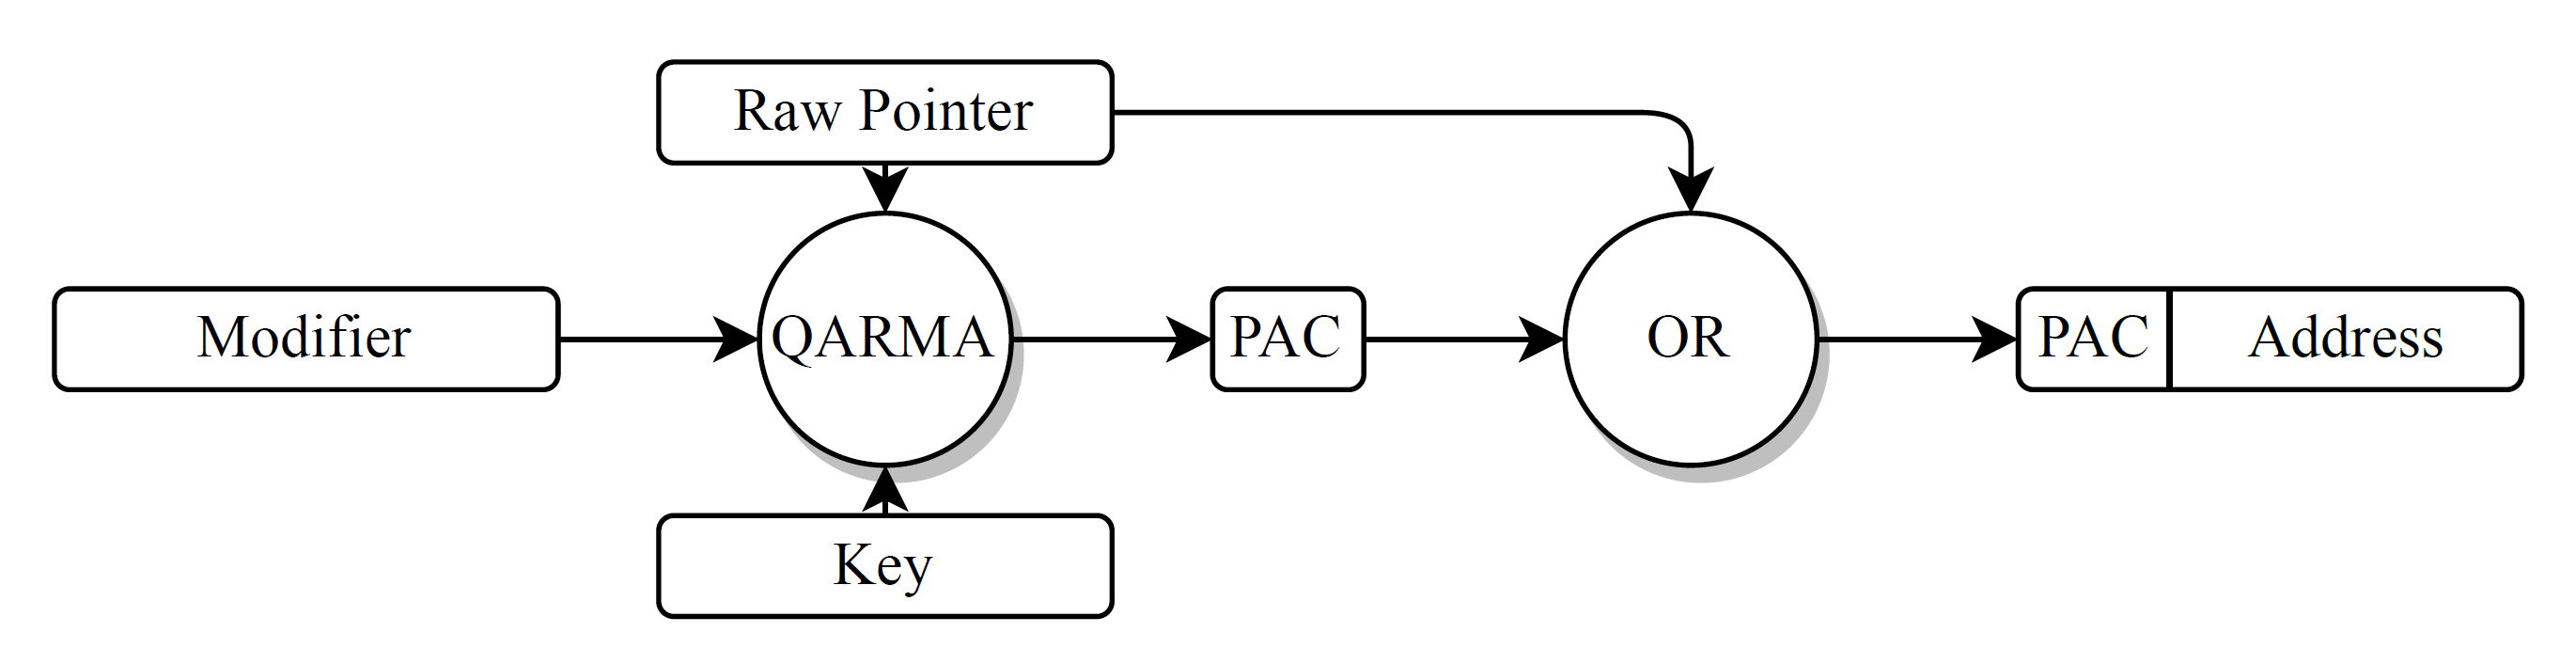
\includegraphics[width=0.8\linewidth]{./images/pa.png}
	% 	\caption{Existing mechanisms are not enough to defeat DMA attacks.}
	% \end{figure}
\end{frame}

% \section{Background}
% \begin{frame}
% 	\frametitle{Existing Mechanisms}
% 	\begin{figure}
% 		\centering
% 		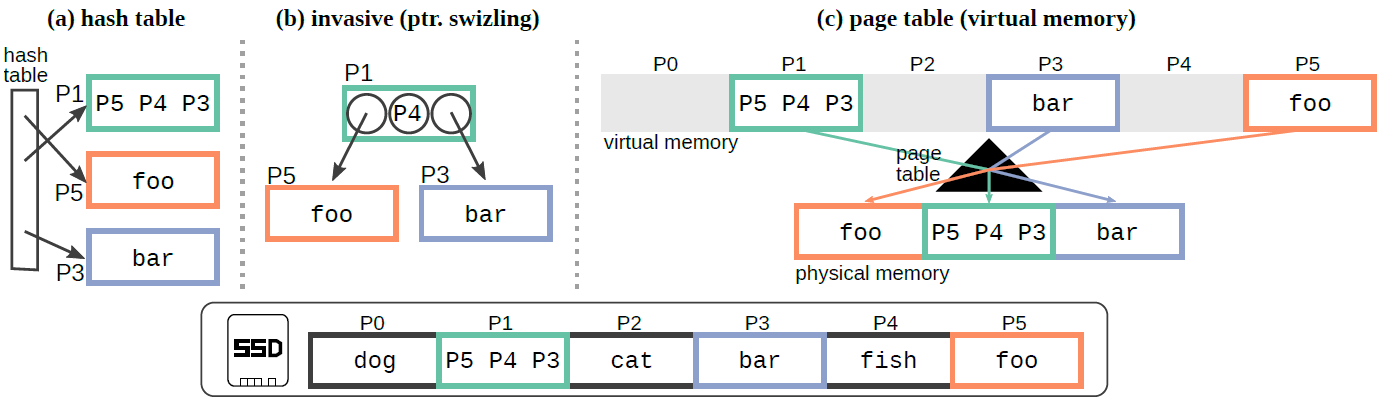
\includegraphics[width=13cm]{./images/existing.png}
% 		\caption{caption}
% 	\end{figure}
% \end{frame}

% \begin{frame}{Design: vmcache (cont.)}
% 	\begin{figure}
% 		\centering
% 		\begin{subfigure}{0.65\linewidth}
% 			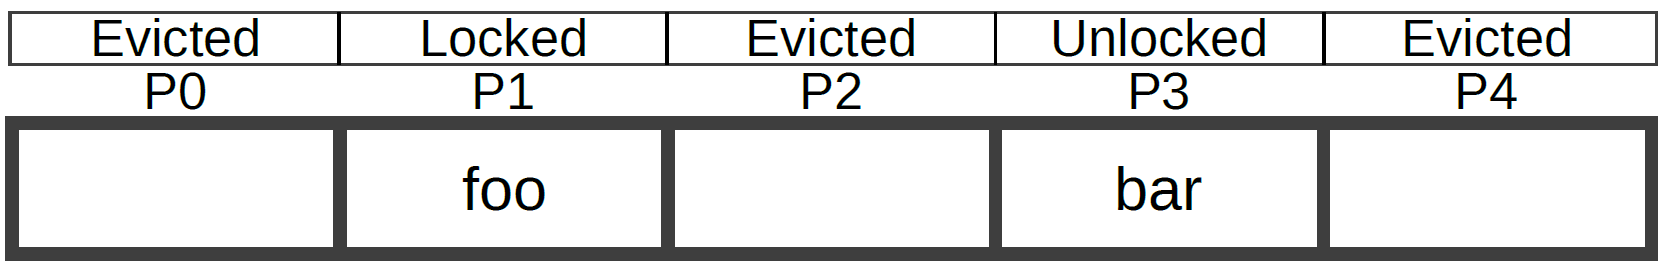
\includegraphics[width=\linewidth]{./images/states.png}
% 			\caption{subcaption}
% 		\end{subfigure}
% 		\begin{subfigure}{0.28\linewidth}
% 			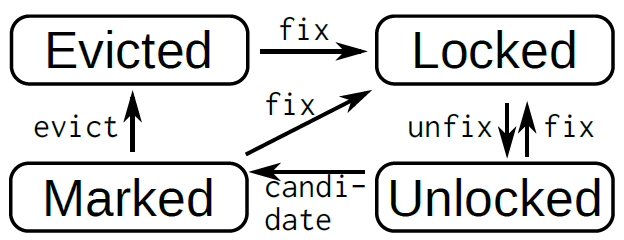
\includegraphics[width=\linewidth]{./images/transfer.png}
% 			\caption{subcaption}
% 		\end{subfigure}
% 		\caption{caption}
% 	\end{figure}
% \end{frame}

% \section{References}
% \begin{frame}{References}
% 	\begin{thebibliography}{99}
% 		\bibitem{zhao1} Yi~Zhao, {\sl An introduction to X}, Sep.~15, 2015
% 		\bibitem{qian2} Er~Qian, San~Sun,
% 		Phys.\ Lett.\ A {\bf xx}, 2xx (20xx)
% 		\bibitem{li4} Si~Li, Phys.\ Rev.\ C {\bf xx}, 5xx (20xx)

% 	\end{thebibliography}
% \end{frame}

\end{document}